\documentclass[xetex,mathserif,serif]{beamer}
\usepackage{polyglossia}
\setdefaultlanguage[babelshorthands=true]{russian}
\usepackage{minted}
\usepackage{tabu}

\useoutertheme{infolines}

\usepackage{fontspec}
\setmainfont{FreeSans}
\newfontfamily{\russianfonttt}{FreeSans}

\usepackage{textpos}
\setlength{\TPHorizModule}{1cm}
\setlength{\TPVertModule}{1cm}

\setbeamertemplate{blocks}[rounded][shadow=false]

\setbeamercolor*{block title alerted}{fg=red!50!black,bg=red!20}
\setbeamercolor*{block body alerted}{fg=black,bg=red!10}

\tabulinesep=1.2mm

\title[Моделирование поведения]{Лекция 5: Моделирование поведения}
\author[Юрий Литвинов]{Юрий Литвинов\\\small{\textcolor{gray}{yurii.litvinov@gmail.com}}}
\date{19.10.2017г}

\newcommand{\todo}[1] {
	\begin{center}\textcolor{red}{TODO: #1}\end{center}
}

\newcommand{\DownArrow} {
	\hspace{2cm}\begin{LARGE}$\downarrow$\end{LARGE}
}

\newcommand{\attribution}[1] {
	\vspace{-5mm}\begin{flushright}\begin{scriptsize}\textcolor{gray}{\textcopyright\, #1}\end{scriptsize}\end{flushright}
}

\begin{document}

	\frame{\titlepage}

	\section{Диаграммы состояний}

	\begin{frame}
		\frametitle{Диаграммы конечных автоматов}
		\framesubtitle{Диаграммы состояний}
		\begin{columns}
			\begin{column}{0.5\textwidth}
				\begin{itemize}
					\item Состояния объекта как часть жизненного цикла
					\item Моделирование реактивных объектов
					\begin{itemize}
						\item Например, сетевое соединение
						\item Или знакомый пример с торговым автоматом
					\end{itemize}
					\item Имеют исполнимую семантику
					\item Д. Харел, 1987
				\end{itemize}
			\end{column}
			\begin{column}{0.5\textwidth}
				\begin{center}
					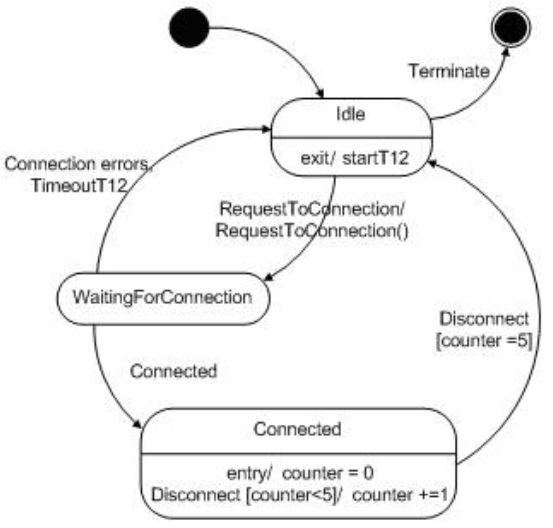
\includegraphics[width=0.7\textwidth]{stateTransitionExample.png}
				\end{center}
			\end{column}
		\end{columns}
	\end{frame}

	\begin{frame}
		\frametitle{Диаграммы конечных автоматов, синтаксис}
		\begin{columns}
			\begin{column}{0.5\textwidth}
				\begin{itemize}
					\item Состояние
					\begin{itemize}
						\item entry activity
						\item exit activity
						\item do activity
						\item внутренний переход
					\end{itemize}
					\item Событие
					\item Переход
					\begin{itemize}
						\item имя события (список параметров) [сторожевое условие] выражение действия
					\end{itemize}
				\end{itemize}
			\end{column}
			\begin{column}{0.5\textwidth}
				\begin{center}
					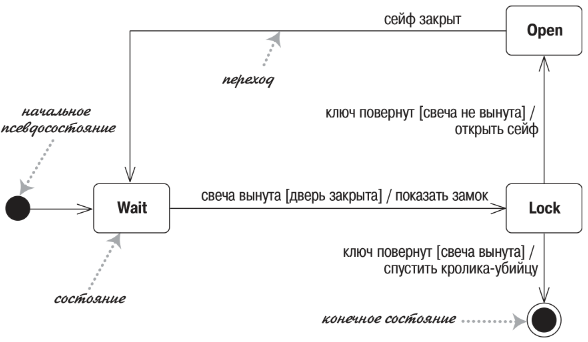
\includegraphics[width=\textwidth]{stateTransitionSyntax.png}
					\attribution{М. Фаулер, UML. Основы}
				\end{center}
			\end{column}
		\end{columns}
	\end{frame}

	\begin{frame}
		\frametitle{Пример, мобильный телефон}
		\begin{center}
			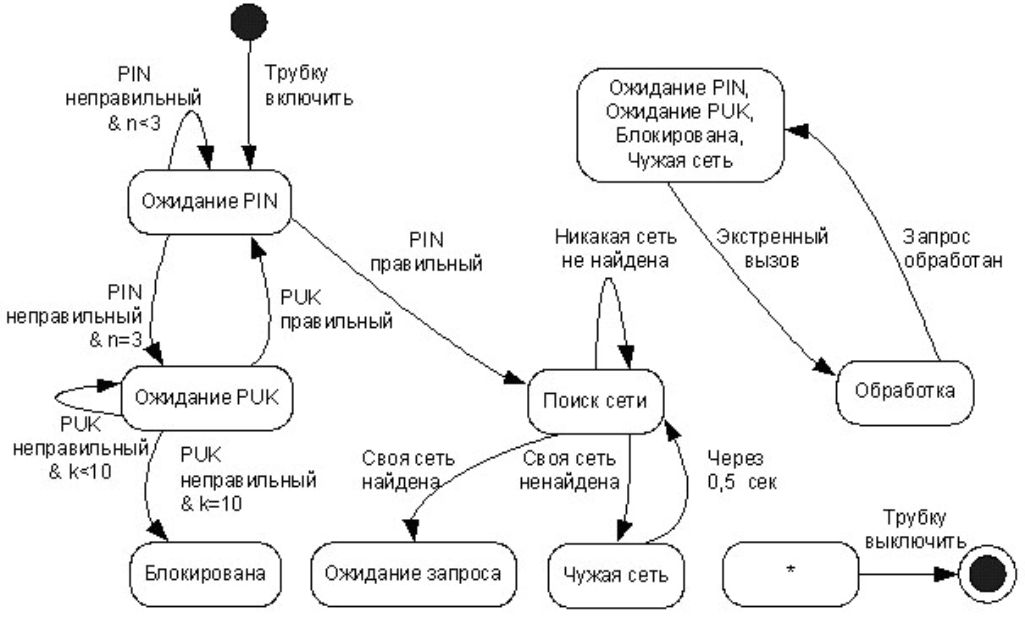
\includegraphics[width=0.7\textwidth]{stateTransitionExample2.png}
		\end{center}
	\end{frame}

	\begin{frame}
		\frametitle{Диаграммы конечных автоматов, прочие вещи}
		Активности:
		\begin{columns}
			\begin{column}{0.5\textwidth}
				\begin{center}
					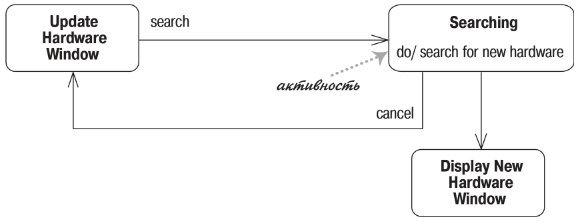
\includegraphics[width=\textwidth]{stateTransitionInternalEventExample.png}
				\end{center}
			\end{column}
			\begin{column}{0.5\textwidth}
				\begin{center}
					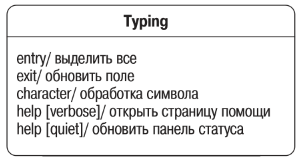
\includegraphics[width=0.5\textwidth]{stateTransitionInternalEvents.png}
				\end{center}
			\end{column}
		\end{columns}

		\begin{columns}
			\begin{column}{0.5\textwidth}
				Вложенные состояния:
				\begin{center}
					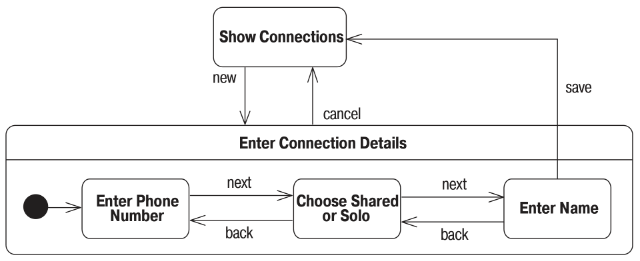
\includegraphics[width=\textwidth]{stateTransitionNestedStates.png}
					\attribution{М. Фаулер, UML. Основы}
				\end{center}
			\end{column}
			\begin{column}{0.5\textwidth}
				Параллельные состояния, псевдосостояние истории:
				\begin{center}
					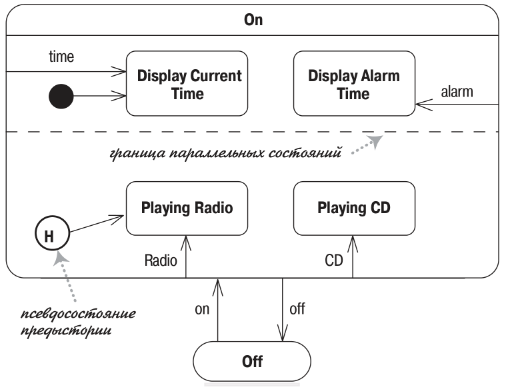
\includegraphics[width=0.7\textwidth]{stateTransitionParallelStates.png}
				\end{center}
			\end{column}
		\end{columns}
	\end{frame}

	\begin{frame}[fragile]
		\frametitle{Генерация кода}
		\begin{columns}
			\begin{column}{0.5\textwidth}
				\begin{tiny}
					\begin{minted}{java}
public void handleEvent(PanelEvent anEvent) {
    switch (currentState) {
        case PanelState.Open:
            switch (anEvent) {
                case PanelEvent.SafeClosed:
                    currentState = PanelState.Wait;
            }
            break;
        case PanelState.Wait:
            switch (anEvent) {
                case PanelEvent.CandleRemoved:
                    if (isDoorOpen) {
                        revealLock();
                        currentState = PanelState.Lock;
                    }
            }
            break;
        case PanelState.Lock:
            switch (anEvent) {
                case PanelEvent.KeyTurned:
                    if (isCandleIn) {
                        openSafe();
                        currentState = PanelState.Open;
                    } else {
                        releaseKillerRabbit();
                        currentState = PanelState.Final;
                    }
            }
            break;
    }
}
					\end{minted}
				\end{tiny}
			\end{column}
			\begin{column}{0.5\textwidth}
				\begin{center}
					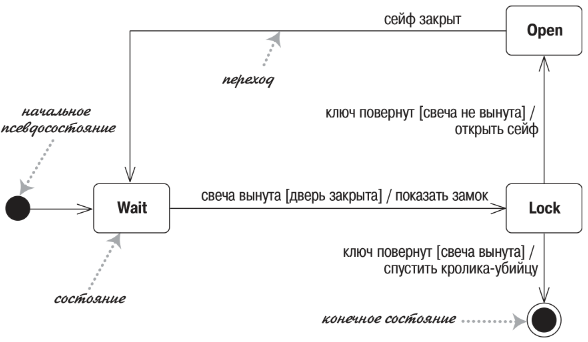
\includegraphics[width=\textwidth]{stateTransitionSyntax.png}
					\attribution{М. Фаулер, UML. Основы}
				\end{center}
			\end{column}
		\end{columns}
	\end{frame}

	\begin{frame}
		\frametitle{Таблица состояний}
		\begin{center}
			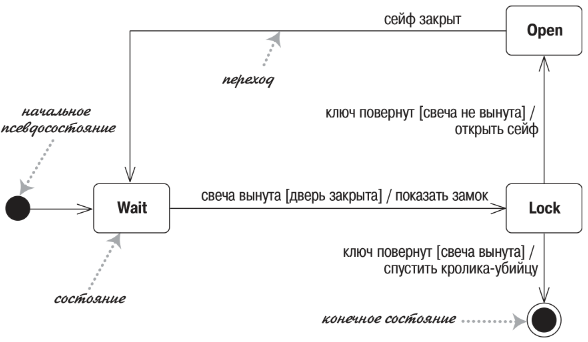
\includegraphics[width=0.4\textwidth]{stateTransitionSyntax.png}
		\end{center}

		\begin{center}
			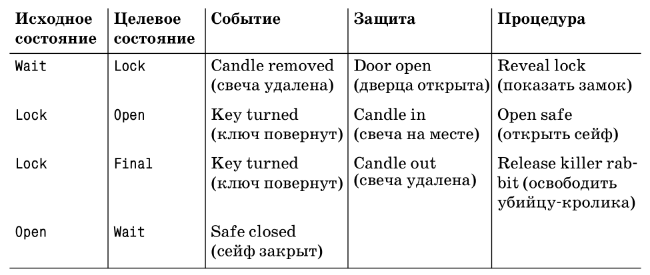
\includegraphics[width=0.5\textwidth]{stateTransitionStateTable.png}
			\attribution{М. Фаулер, UML. Основы}
		\end{center}
	\end{frame}

	\begin{frame}
		\frametitle{Паттерн ``Состояние''}
		\begin{center}
			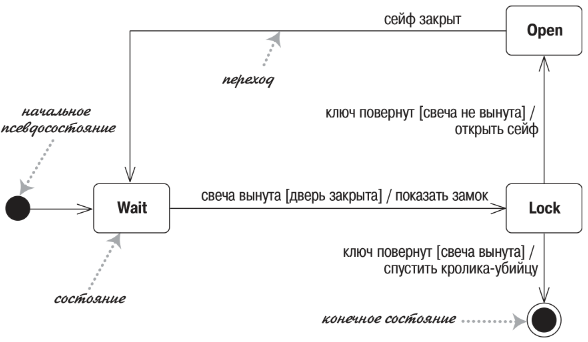
\includegraphics[width=0.4\textwidth]{stateTransitionSyntax.png}
		\end{center}

		\begin{center}
			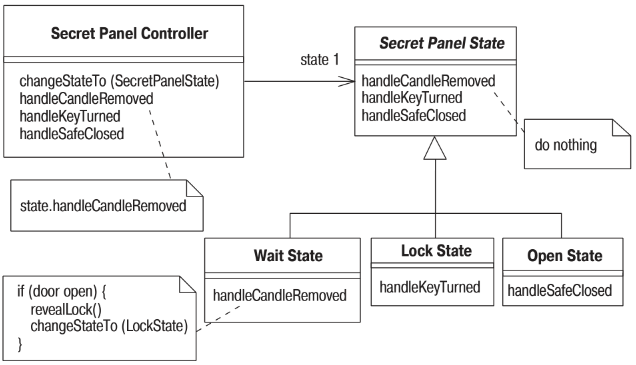
\includegraphics[width=0.5\textwidth]{stateTransitionStatePattern.png}
			\attribution{М. Фаулер, UML. Основы}
		\end{center}
	\end{frame}

	\section{Диаграммы последовательностей}

	\begin{frame}
		\frametitle{Диаграммы последовательностей}
		\begin{columns}
			\begin{column}{0.5\textwidth}
				\begin{itemize}
					\item Применяются для визуализации взаимодействия между объектами
					\begin{itemize}
						\item Особо удобно для асинхронных вызовов
						\item Телекоммуникационные протоколы
					\end{itemize}
					\item Могут применяться на этапе анализа предметной области
					\item Могут применяться для составления плана тестирования
					\item И даже для визуализации логов работающей системы
				\end{itemize}
			\end{column}
			\begin{column}{0.5\textwidth}
				\begin{center}
					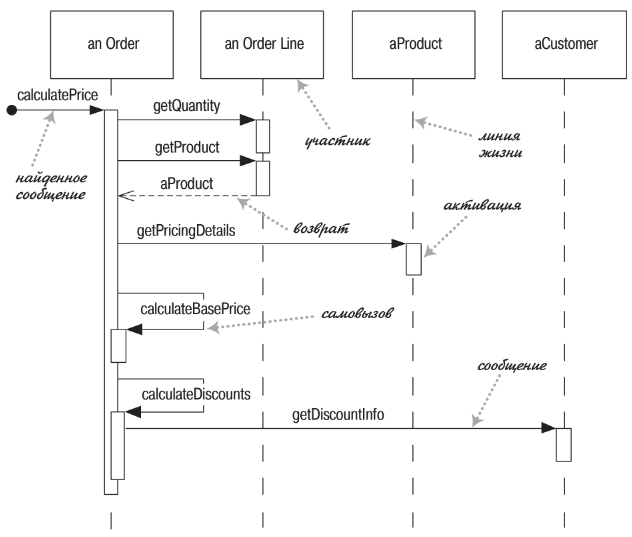
\includegraphics[width=0.9\textwidth]{sequenceDiagramSyntax.png}
					\attribution{М. Фаулер, UML. Основы}
				\end{center}
			\end{column}
		\end{columns}
	\end{frame}

	\begin{frame}
		\frametitle{Ещё немного о синтаксисе}
		\begin{center}
			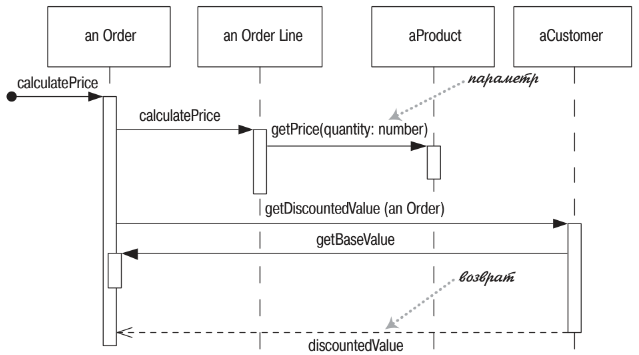
\includegraphics[width=0.6\textwidth]{sequenceDiagramSyntax2.png}
			\attribution{М. Фаулер, UML. Основы}
		\end{center}
	\end{frame}

	\begin{frame}
		\frametitle{Пример}
		\begin{center}
			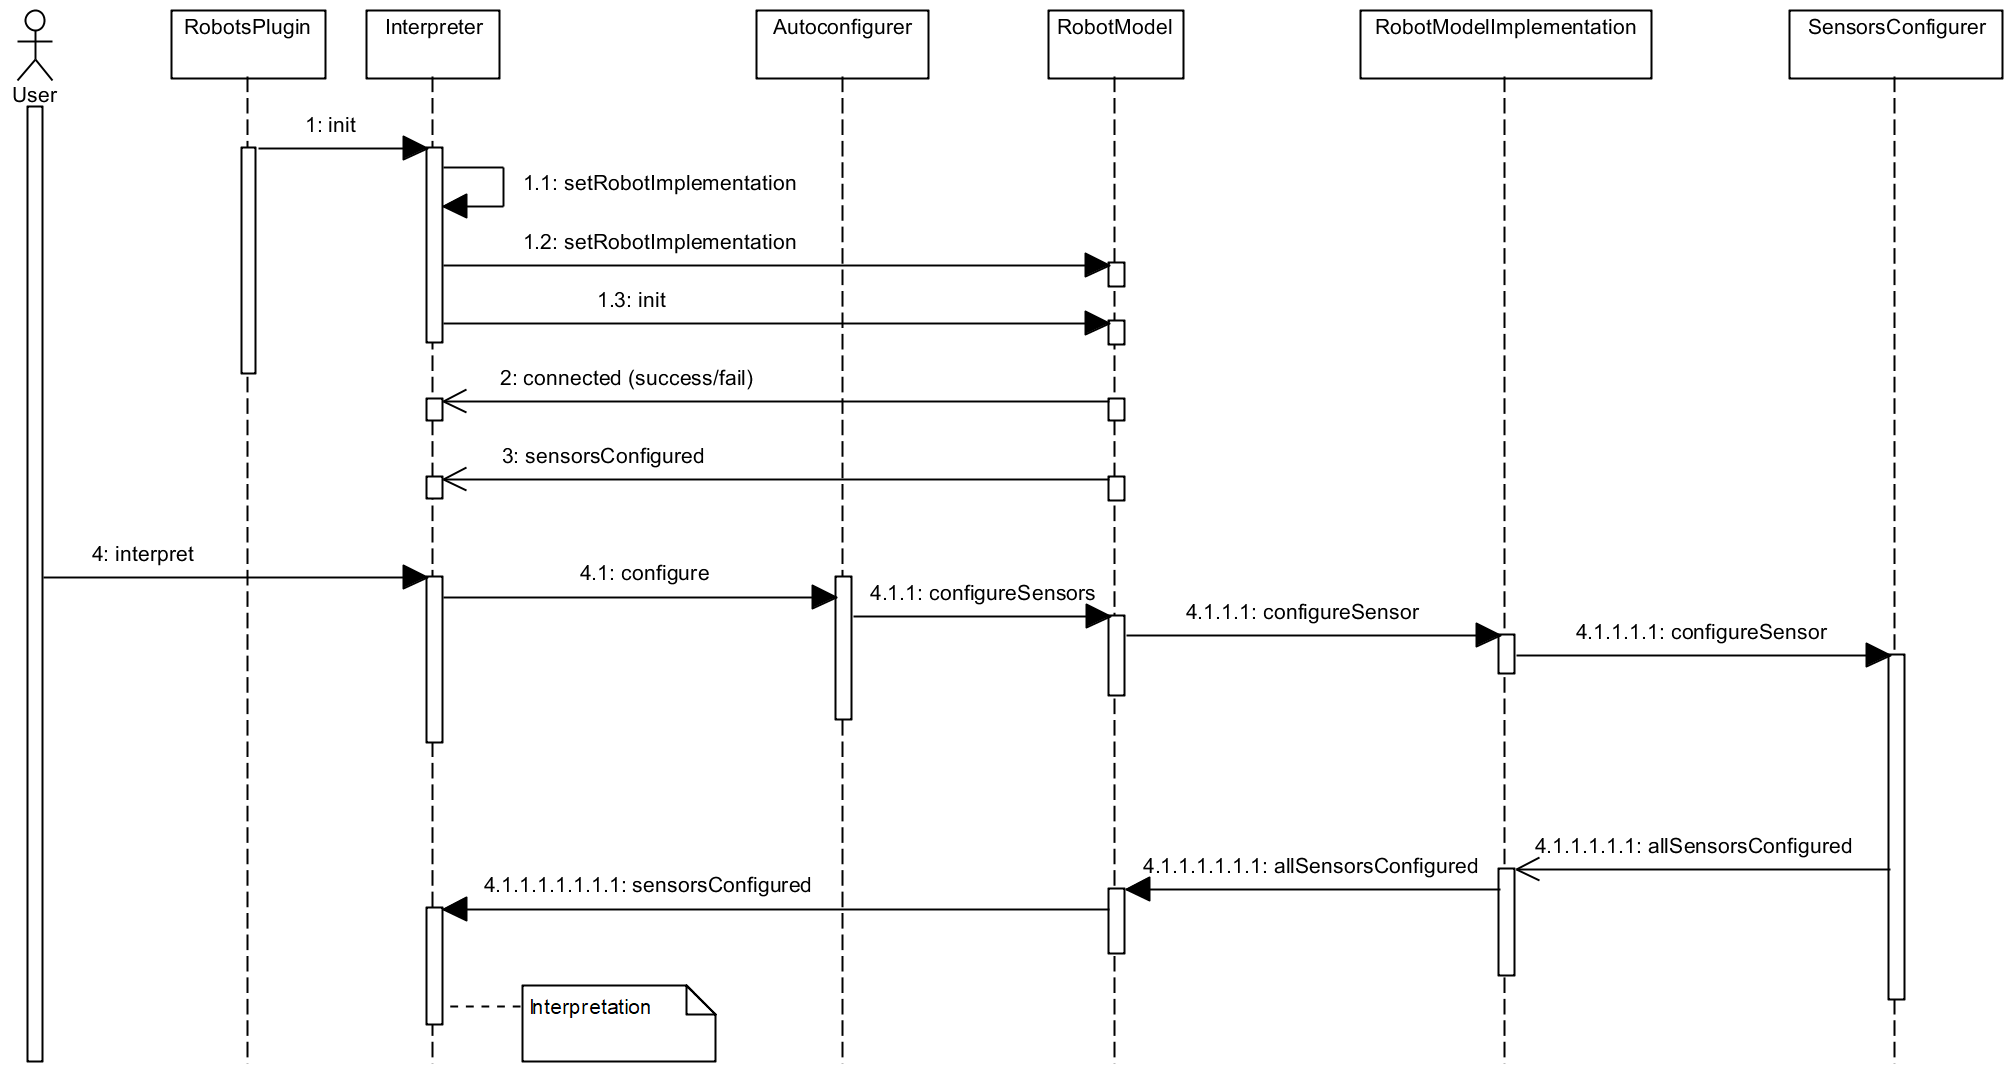
\includegraphics[width=\textwidth]{sequenceDiagramExample.png}
		\end{center}
	\end{frame}

	\begin{frame}
		\frametitle{Ещё пример}
		\begin{center}
			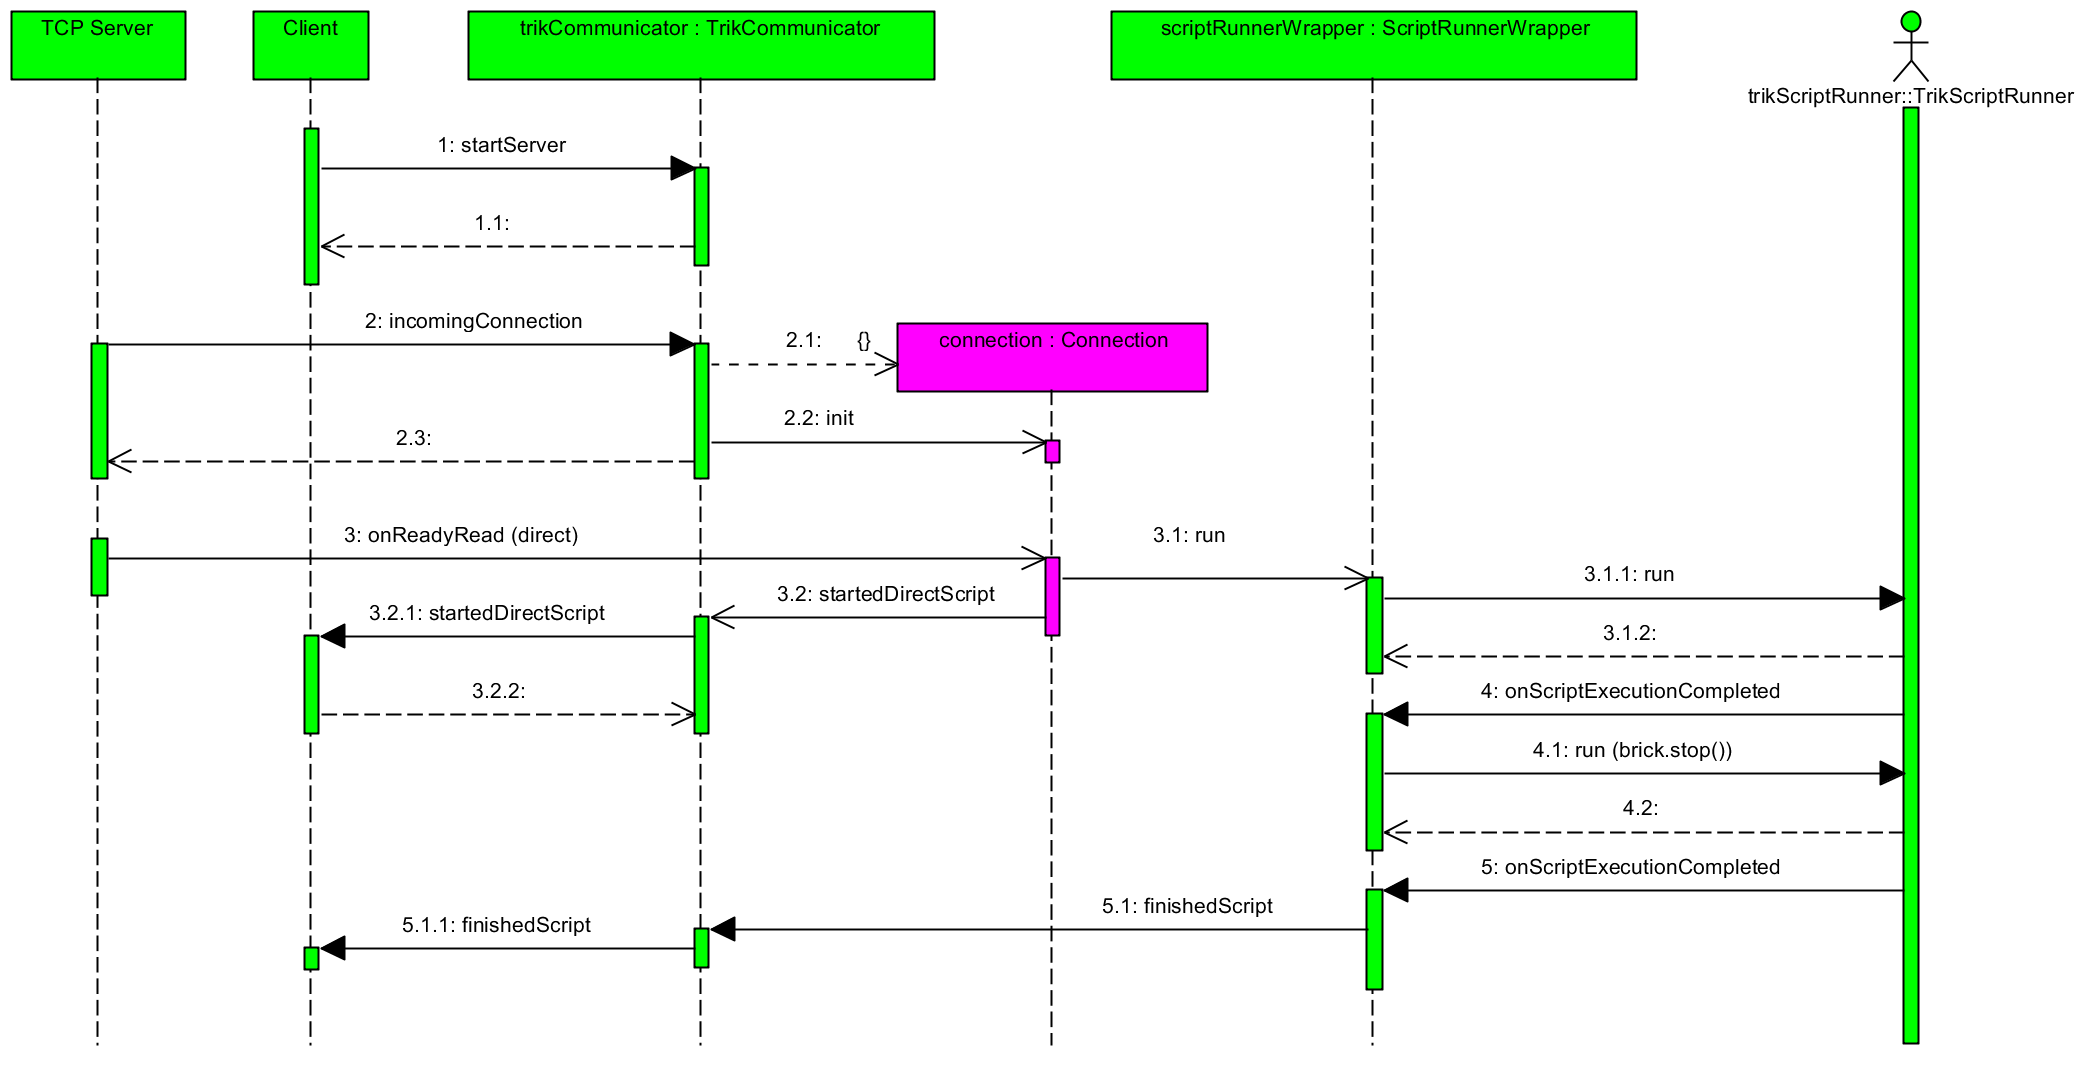
\includegraphics[width=\textwidth]{sequenceDiagramExample2.png}
		\end{center}
	\end{frame}

	\begin{frame}
		\frametitle{И ещё пример}
		\begin{center}
			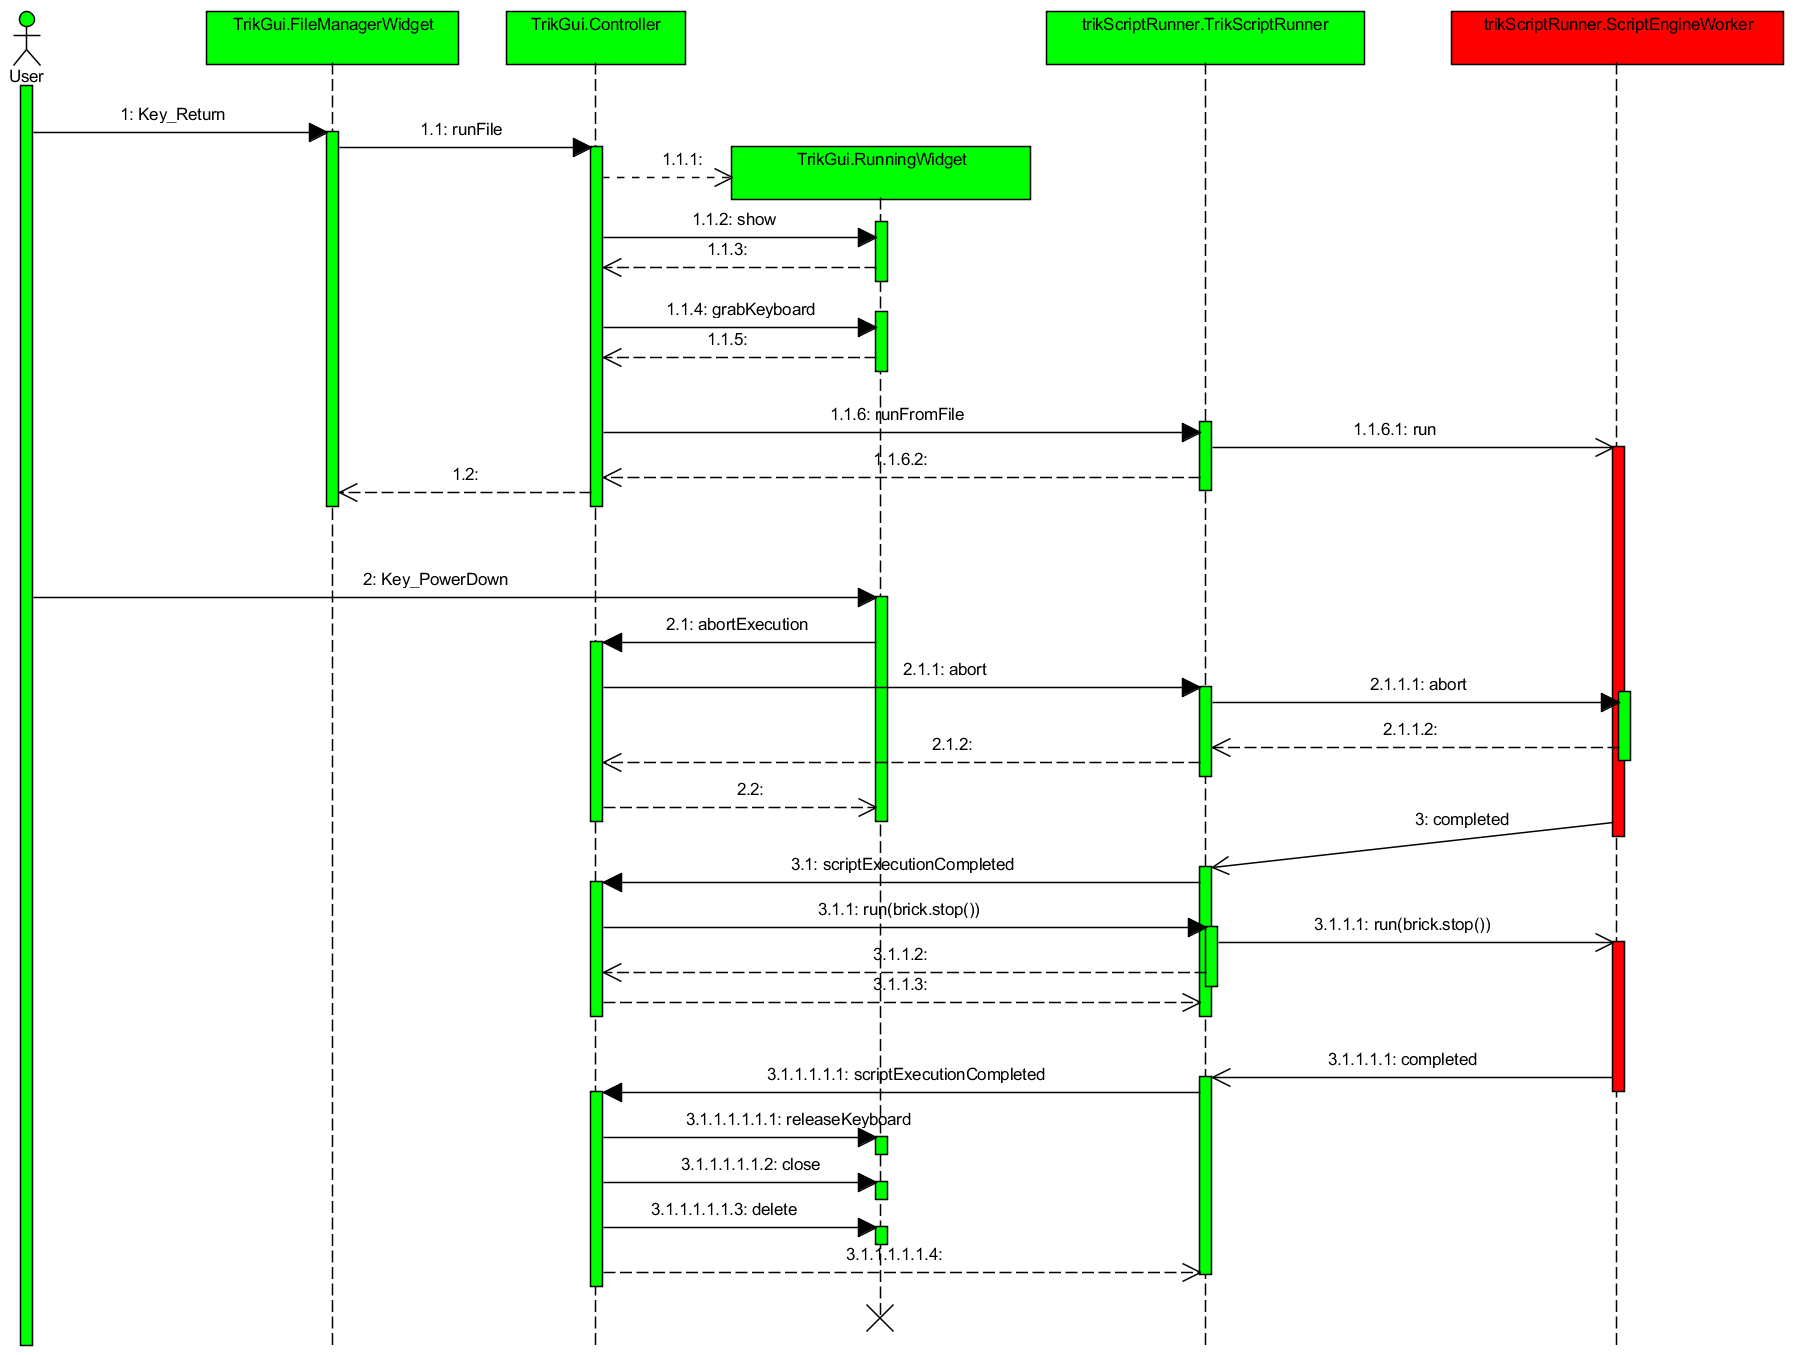
\includegraphics[width=0.8\textwidth]{sequenceDiagramExample3.png}
		\end{center}
	\end{frame}

	\begin{frame}
		\frametitle{Создание и удаление объектов}
		\begin{center}
			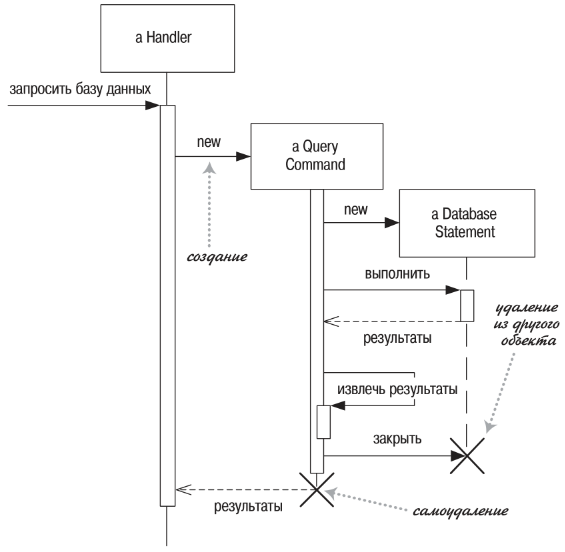
\includegraphics[width=0.5\textwidth]{sequenceDiagramCreationAndDeletion.png}
			\attribution{М. Фаулер, UML. Основы}
		\end{center}
	\end{frame}

	\begin{frame}[fragile]
		\frametitle{Фреймы}
		\begin{columns}
			\begin{column}{0.5\textwidth}
				\begin{small}
					\begin{minted}{text}
    foreach (lineitem)
        if (product.value > $10K)
            careful.dispatch
        else
            regular.dispatch
        end if
    end for
    if (needsConfirmation) 
        messenger.confirm
					\end{minted}
				\end{small}
			\end{column}
			\begin{column}{0.5\textwidth}
				\begin{center}
					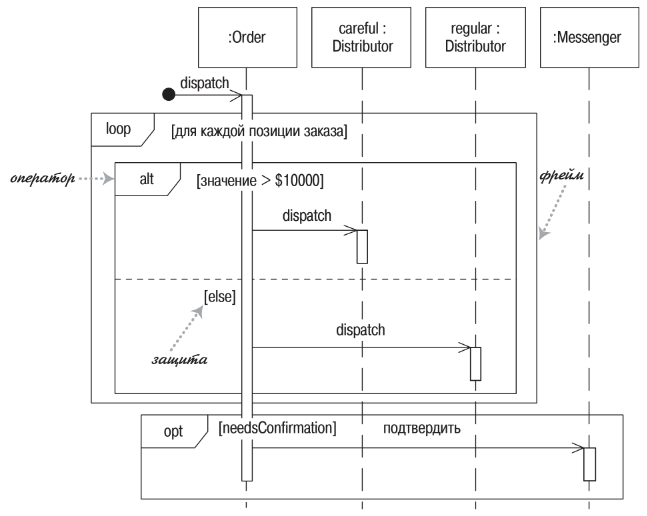
\includegraphics[width=\textwidth]{sequenceDiagramFrames.png}
					\attribution{М. Фаулер, UML. Основы}
				\end{center}
			\end{column}
		\end{columns}
	\end{frame}

	\section{Коммуникационные диаграммы}

	\begin{frame}
		\frametitle{Коммуникационные диаграммы}
		\begin{columns}
			\begin{column}{0.5\textwidth}
				\begin{itemize}
					\item Применяются для визуализации взаимодействия между объектами
					\begin{itemize}
						\item Более легковесный аналог диаграмм последовательностей
						\item Тоже отображают один сценарий взаимодействия
					\end{itemize}
				\end{itemize}
			\end{column}
			\begin{column}{0.5\textwidth}
				\begin{center}
					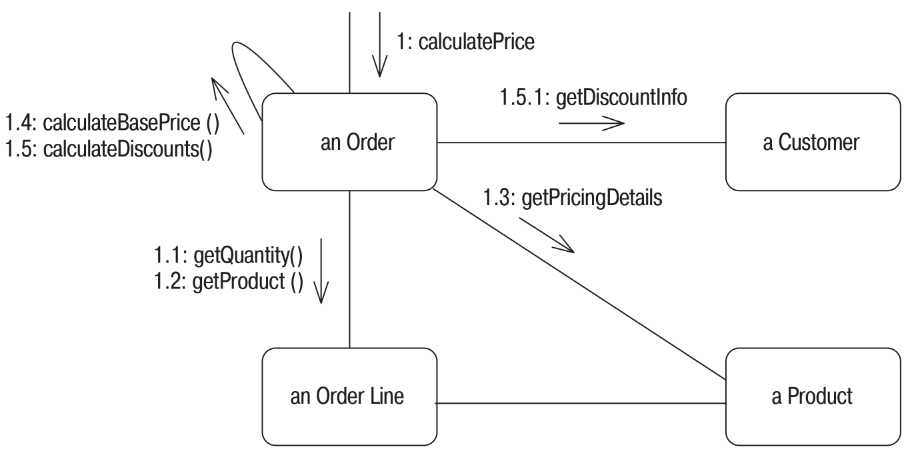
\includegraphics[width=\textwidth]{communicationDiagram.png}
					\attribution{М. Фаулер, UML. Основы}
				\end{center}
			\end{column}
		\end{columns}
	\end{frame}

	\begin{frame}
		\frametitle{Коммуникационные диаграммы, пример}
		\begin{center}
			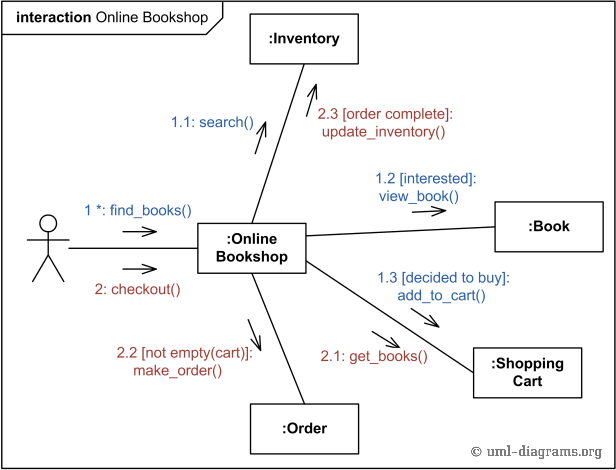
\includegraphics[width=0.6\textwidth]{communicationDiagramExample.png}
			\attribution{http://www.uml-diagrams.org/}
		\end{center}
	\end{frame}

	\section{Диаграммы составных структур}

	\begin{frame}
		\frametitle{Диаграммы составных структур}
		\begin{columns}
			\begin{column}{0.5\textwidth}
				\begin{itemize}
					\item По сути, продвинутые диаграммы компонентов
					\item Внутри компоненты не другие компоненты, а части (роли)
				\end{itemize}
				\vspace{3mm}
				\begin{center}
					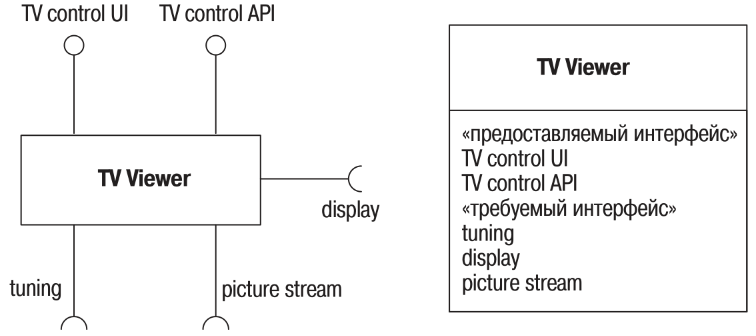
\includegraphics[width=0.9\textwidth]{compositeStructureElement.png}
				\end{center}
			\end{column}
			\begin{column}{0.5\textwidth}
				\begin{center}
					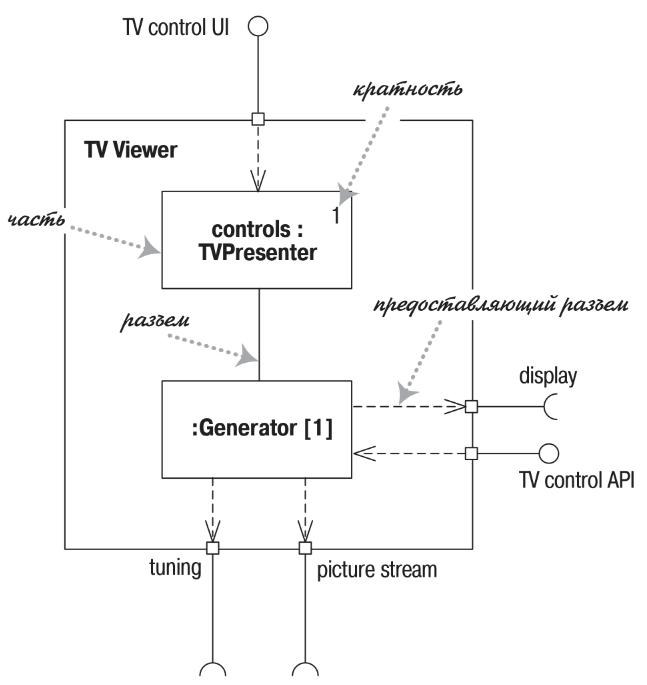
\includegraphics[width=0.8\textwidth]{compositeStructureDiagram.png}
					\attribution{М. Фаулер, UML. Основы}
				\end{center}
			\end{column}
		\end{columns}
	\end{frame}

	\begin{frame}
		\frametitle{Диаграммы составных структур, пример}
		\begin{center}
			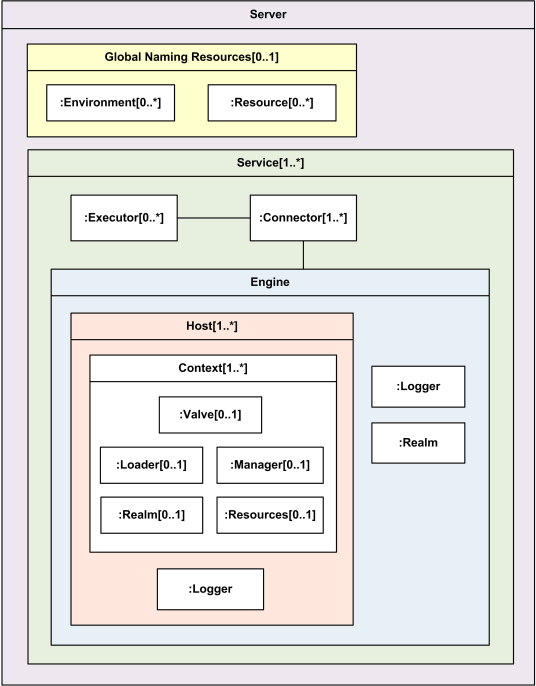
\includegraphics[width=0.45\textwidth]{compositeStructureExample.png}
			\attribution{http://www.uml-diagrams.org/}
		\end{center}
	\end{frame}

	\section{Диаграммы коопераций}

	\begin{frame}
		\frametitle{Диаграммы коопераций}
		\begin{columns}
			\begin{column}{0.5\textwidth}
				\begin{itemize}
					\item Показывают взаимодействие между объектами (ролями) в рамках одного сценария использования
				\end{itemize}
				\vspace{3mm}
				\begin{center}
					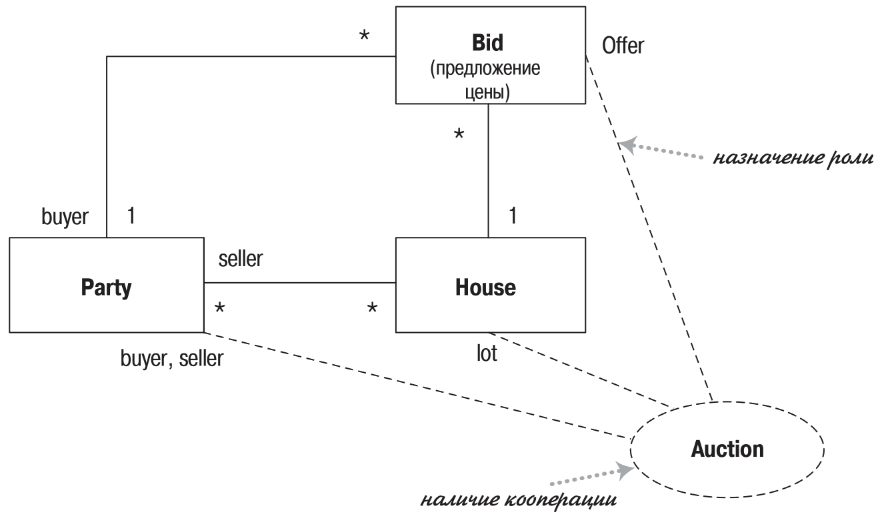
\includegraphics[width=0.9\textwidth]{cooperationAlternateNotation.png}
				\end{center}
			\end{column}
			\begin{column}{0.5\textwidth}
				\begin{center}
					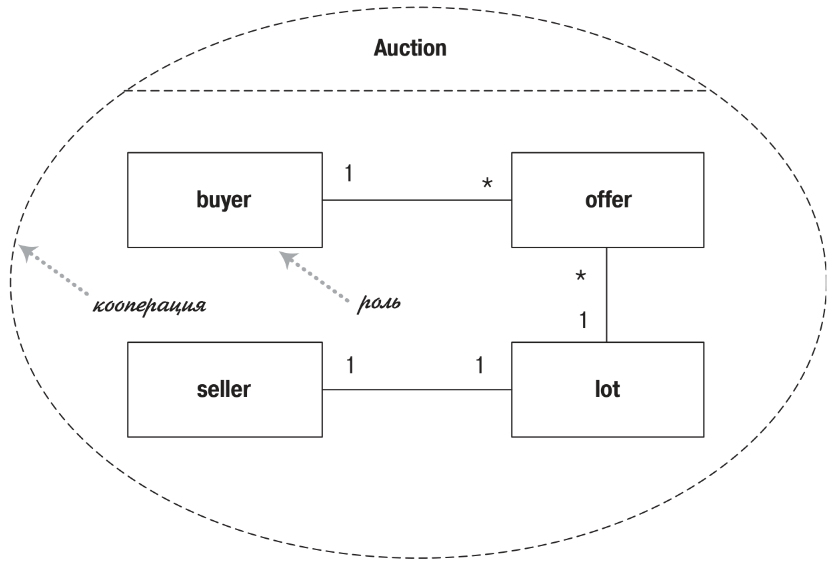
\includegraphics[width=0.9\textwidth]{cooperationDiagram.png}
					\attribution{М. Фаулер, UML. Основы}
				\end{center}
			\end{column}
		\end{columns}
	\end{frame}

	\begin{frame}
		\frametitle{Диаграммы коопераций, последовательности}
		\begin{columns}
			\begin{column}{0.5\textwidth}
				\begin{center}
					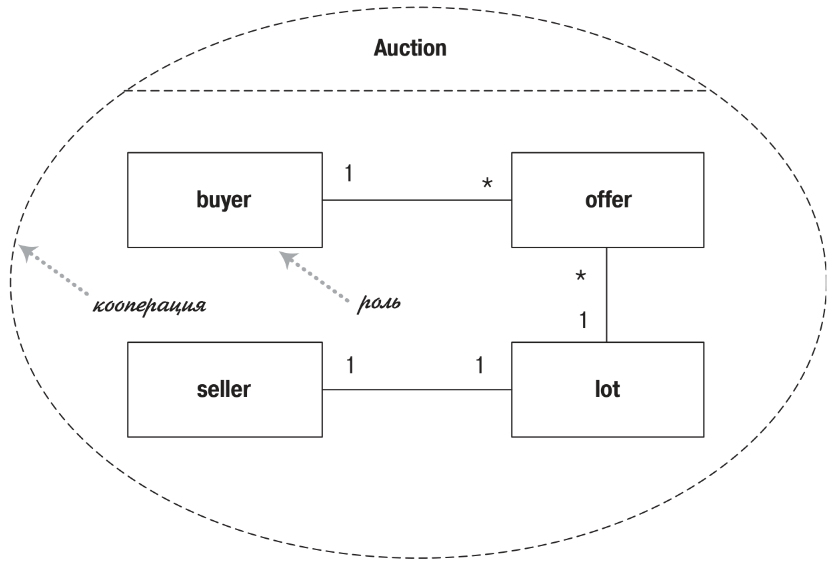
\includegraphics[width=0.9\textwidth]{cooperationDiagram.png}
				\end{center}
			\end{column}
			\begin{column}{0.5\textwidth}
				\begin{center}
					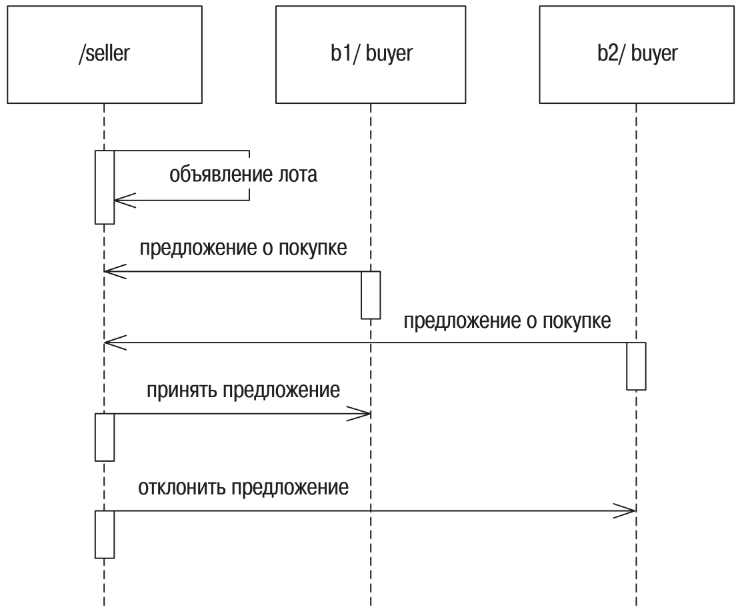
\includegraphics[width=0.9\textwidth]{cooperationSequenceDiagram.png}
					\attribution{М. Фаулер, UML. Основы}
				\end{center}
			\end{column}
		\end{columns}
	\end{frame}

	\section{Временные диаграммы}

	\begin{frame}
		\frametitle{Временные диаграммы}
		\begin{columns}
			\begin{column}{0.5\textwidth}
				\begin{itemize}
					\item Для моделирования временных ограничений в системах реального времени
				\end{itemize}
				\vspace{3mm}
				\begin{center}
					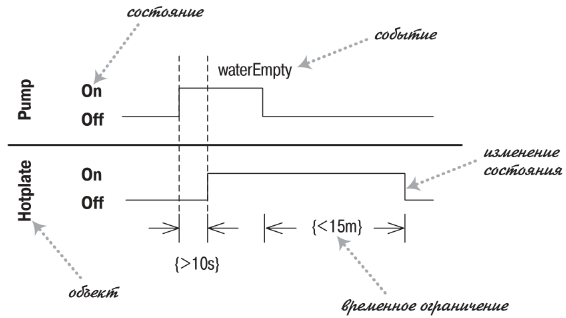
\includegraphics[width=0.9\textwidth]{timingDiagrams.png}
				\end{center}
			\end{column}
			\begin{column}{0.5\textwidth}
				\begin{center}
					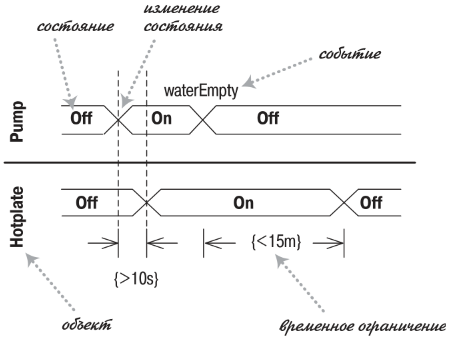
\includegraphics[width=0.8\textwidth]{timingDiagramsAlternate.png}
					\attribution{М. Фаулер, UML. Основы}
				\end{center}
			\end{column}
		\end{columns}
	\end{frame}

	\begin{frame}
		\frametitle{Временная диаграмма, пример}
		\begin{center}
			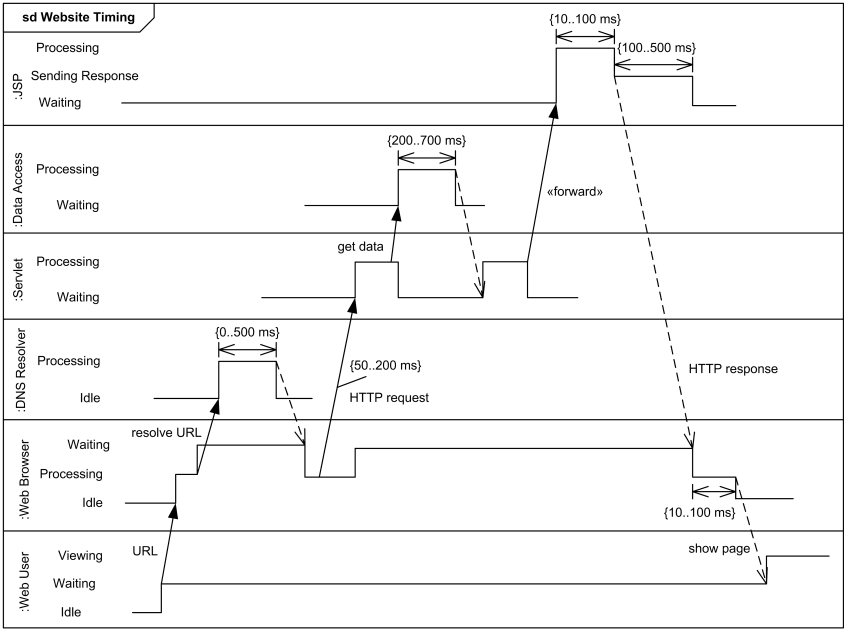
\includegraphics[width=0.7\textwidth]{timingDiagramExample.png}
			\attribution{http://www.uml-diagrams.org/}
		\end{center}
	\end{frame}

	\section{Диаграммы обзора взаимодействия}

	\begin{frame}
		\frametitle{Диаграммы обзора взаимодействия}
		\begin{columns}
			\begin{column}{0.5\textwidth}
				\begin{itemize}
					\item Диаграммы активностей + диаграммы последовательностей
					\item Применяются при наличии взаимодействия со сложной логикой, когда фреймы неудобны
				\end{itemize}
			\end{column}
			\begin{column}{0.5\textwidth}
				\begin{center}
					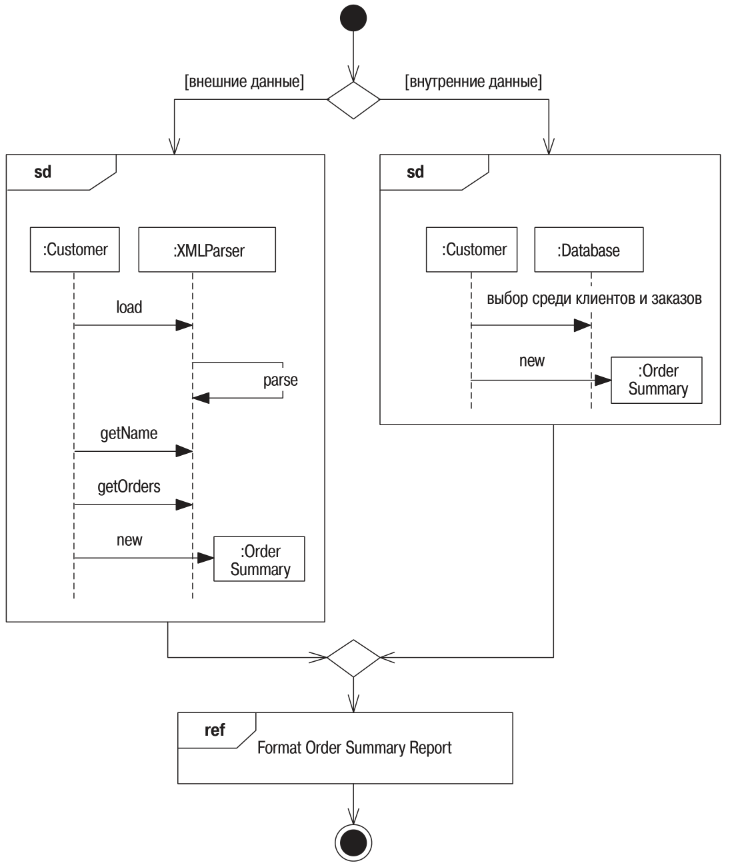
\includegraphics[width=0.9\textwidth]{interactionOverviewDiagrams.png}
					\attribution{М. Фаулер, UML. Основы}
				\end{center}
			\end{column}
		\end{columns}
	\end{frame}

	\begin{frame}
		\frametitle{Диаграмма обзора взаимодействия, пример}
		\begin{center}
			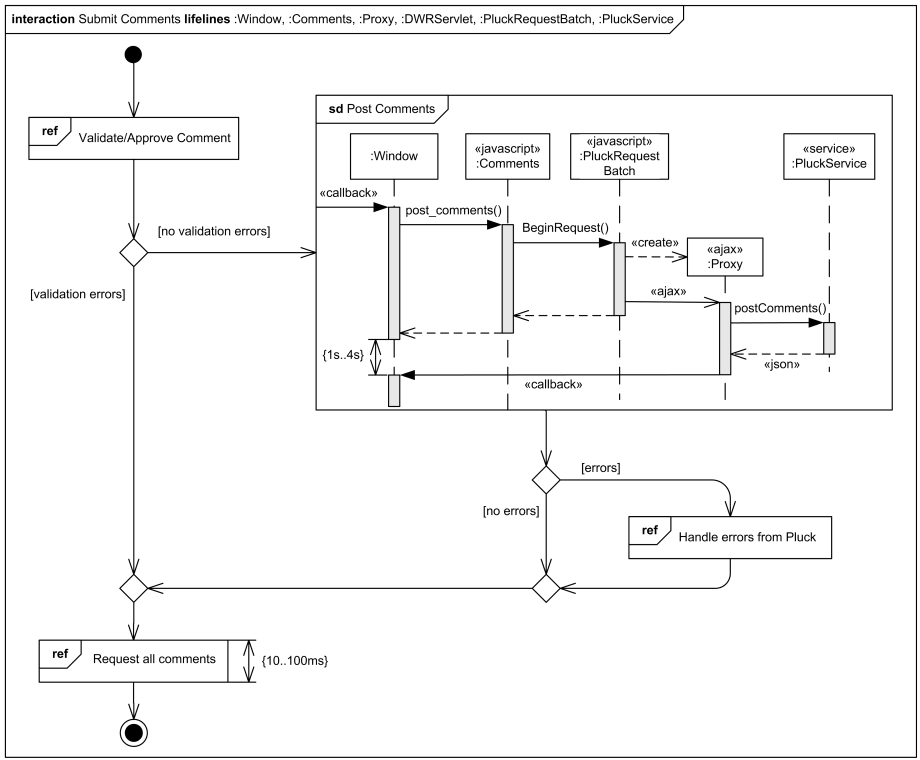
\includegraphics[width=0.7\textwidth]{interactionOverviewExample.png}
			\attribution{http://www.uml-diagrams.org/}
		\end{center}
	\end{frame}

	\section{Диаграммы потоков данных}

	\begin{frame}
		\frametitle{Диаграммы потоков данных}
		\framesubtitle{DFD}
		\begin{columns}
			\begin{column}{0.4\textwidth}
				\begin{itemize}
					\item Показывают обмен данными в системе
					\item Внешние сущности, процессы внутри системы, потоки данных
				\end{itemize}
			\end{column}
			\begin{column}{0.6\textwidth}
				\begin{center}
					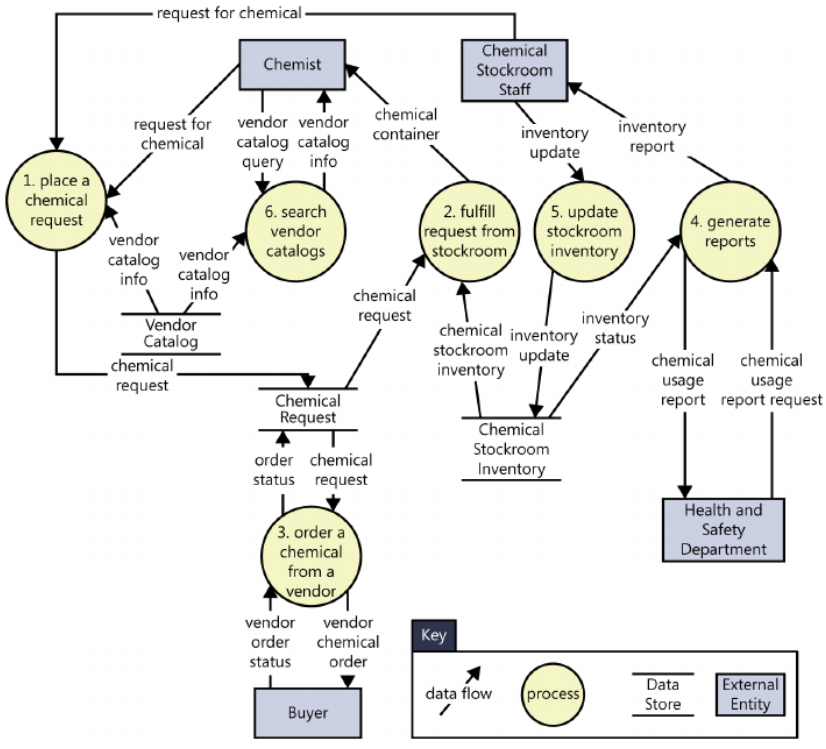
\includegraphics[width=0.9\textwidth]{dfd.png}
				\end{center}
			\end{column}
		\end{columns}
	\end{frame}
	
	\section{Диаграммы IDEF0}
	
	\begin{frame}
		\frametitle{Диаграммы IDEF0}
		\begin{center}
			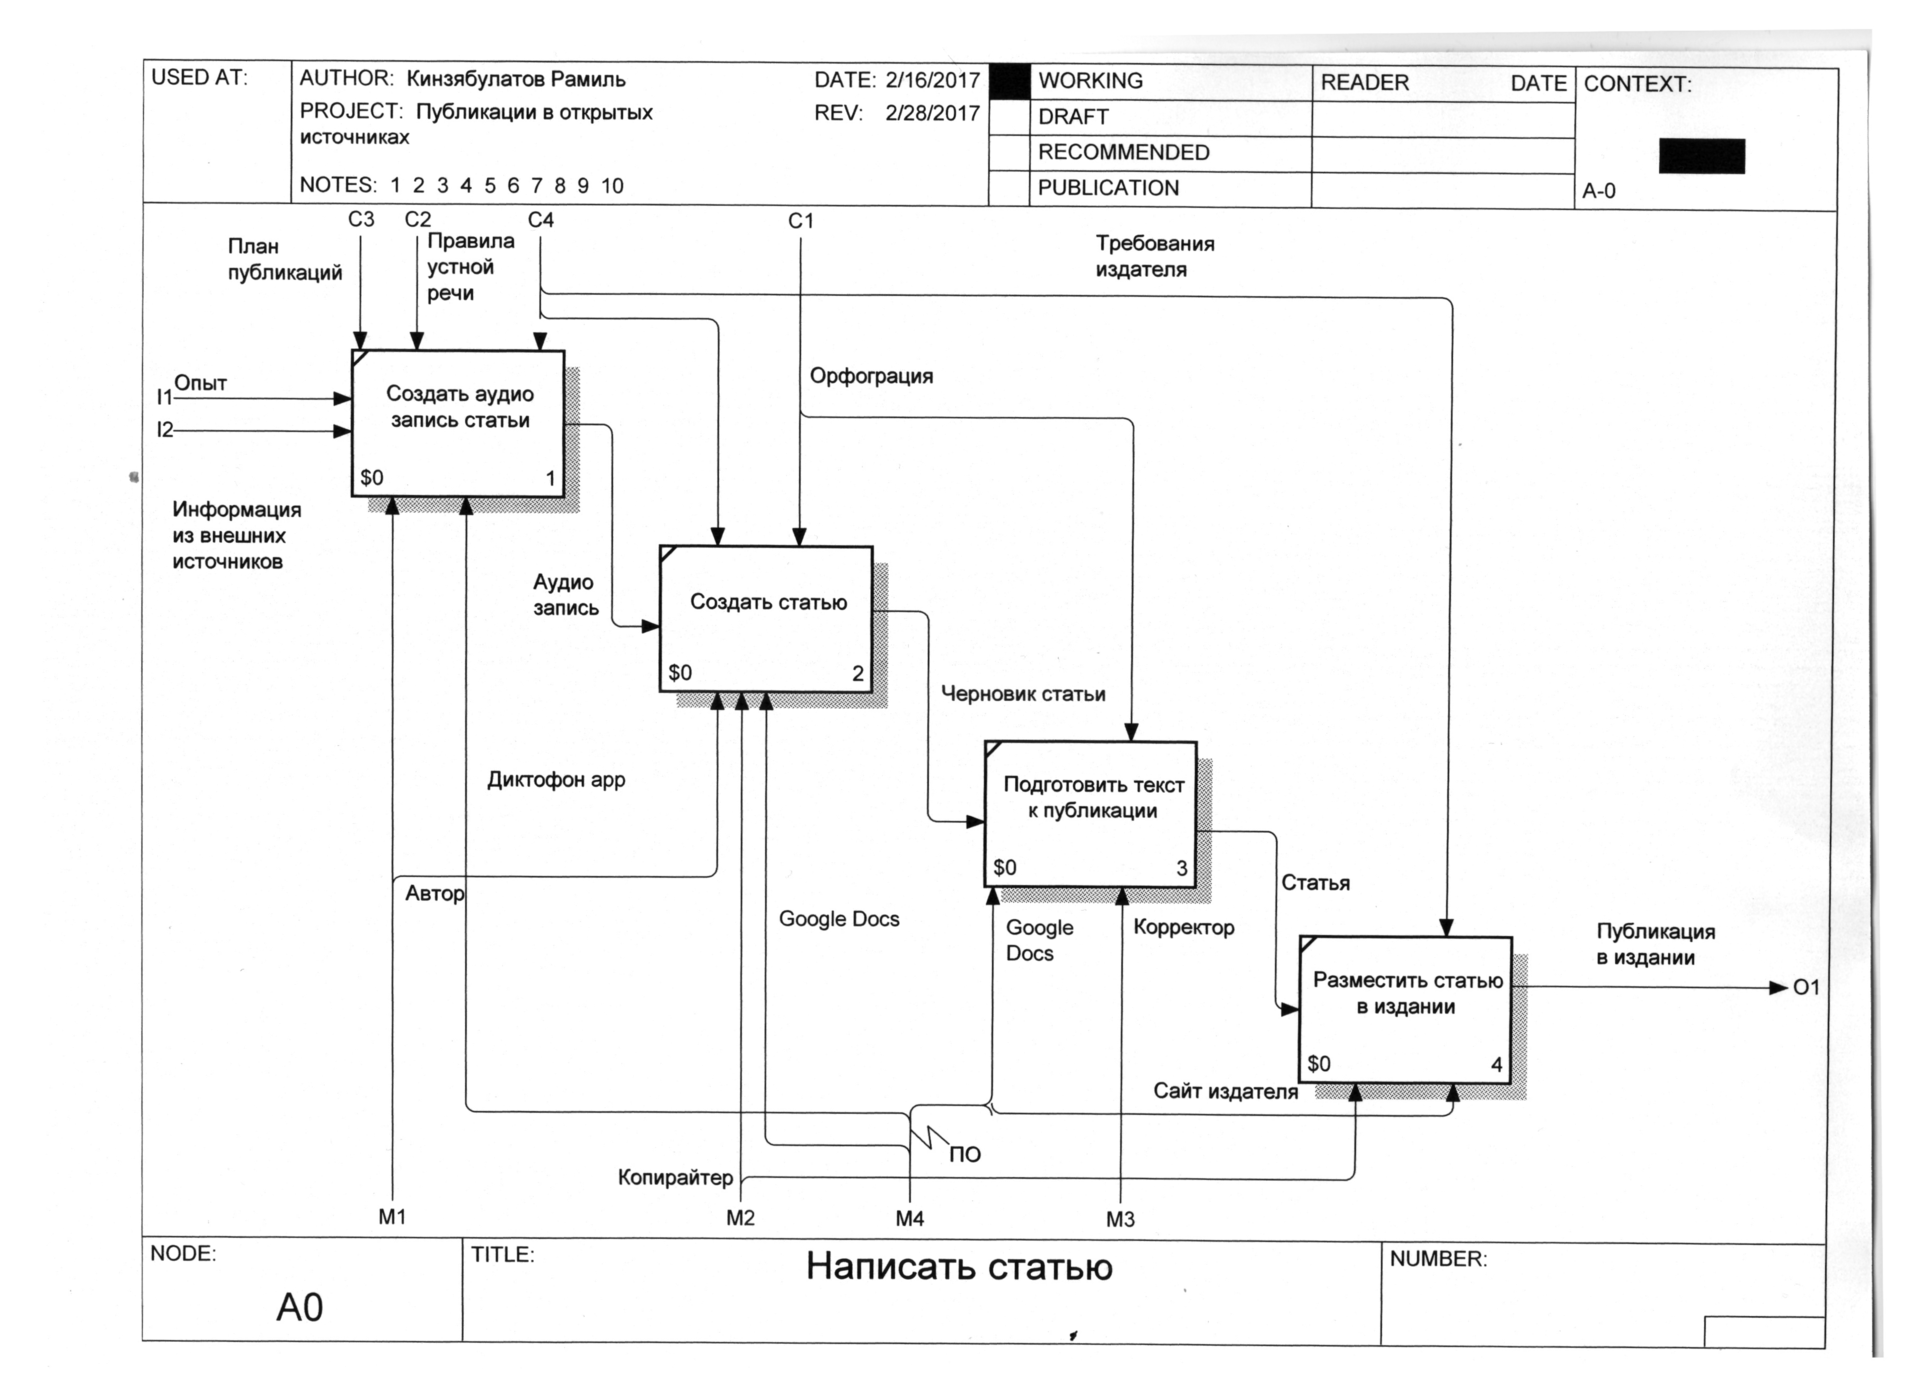
\includegraphics[width=0.80\textwidth]{idef0.png}
			\attribution{https://habrahabr.ru/post/322832/}
		\end{center}
	\end{frame}

	\begin{frame}
		\frametitle{Книжка}
		\begin{columns}
			\begin{column}{0.5\textwidth}
				\begin{center}
					
\includegraphics[width=0.4\textwidth]{umlBookCover.png}
				\end{center}
			\end{column}
			\begin{column}{0.5\textwidth}
				М. Фаулер, UML. Основы. Краткое руководство по стандартному языку объектного моделирования. СПб., Символ-Плюс, 2011. 192 С.
			\end{column}
		\end{columns}
	\end{frame}

\end{document}
